\begin{figure}[htb]
    \centering
    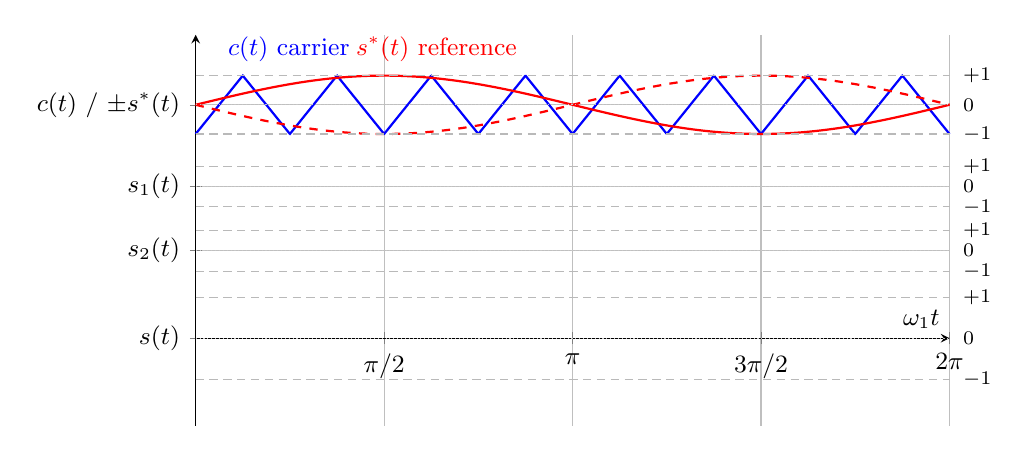
\begin{tikzpicture}
        \begin{axis}[
                xmin=0, xmax=1,
                ymin=-1.5, ymax=5.2,
                width=0.92\textwidth,
                height=0.54\textwidth,
                axis x line=middle,
                axis y line=left,
                grid=major,
                xlabel={$\omega_1 t$},
                ylabel={},
                xtick={0,0.25,0.5,0.75,1},
                xticklabels={$0$,$\pi/2$,$\pi$,$3\pi/2$,$2\pi$},
                ytick={0,1.5,2.6,4},
                yticklabels={$s(t)$,$s_\mathrm{2}(t)$,$s_\mathrm{1}(t)$,{$c(t)$ / $\pm s^*(t)$}},
                ticklabel style={font=\small},
                label style={font=\small},
                samples=200,
                clip=false
            ]
            % Carrier and references (given, lecture convention)
            \addplot[blue, thick, domain=0:1, samples=1200] {4 + 0.5*(1 - 4*abs(mod(8*x,1)-0.5))};
            \addplot[red, thick, domain=0:1, samples=250] {4+0.5*sin(360*x)};
            \addplot[red, dashed, thick, domain=0:1, samples=250] {4-0.5*sin(360*x)};
            \node[anchor=west, font=\small, text=blue] at (axis cs:0.03,4.95) {$c(t)$ carrier};
            \node[anchor=west, font=\small, text=red] at (axis cs:0.2,4.95) {$s^*(t)$ reference};

            % Exact +1/-1 level lines for each signal row
            \addplot[gray!55, densely dashed] coordinates {(0,4.5) (1,4.5)};
            \addplot[gray!55, densely dashed] coordinates {(0,3.5) (1,3.5)};
            \addplot[gray!45, densely dotted] coordinates {(0,4.0) (1,4.0)};
            \addplot[gray!55, densely dashed] coordinates {(0,2.95) (1,2.95)};
            \addplot[gray!55, densely dashed] coordinates {(0,2.25) (1,2.25)};
            \addplot[gray!45, densely dotted] coordinates {(0,2.6) (1,2.6)};
            \addplot[gray!55, densely dashed] coordinates {(0,1.85) (1,1.85)};
            \addplot[gray!55, densely dashed] coordinates {(0,1.15) (1,1.15)};
            \addplot[gray!45, densely dotted] coordinates {(0,1.5) (1,1.5)};
            \addplot[gray!55, densely dashed] coordinates {(0,0.7) (1,0.7)};
            \addplot[gray!55, densely dashed] coordinates {(0,-0.7) (1,-0.7)};
            \addplot[gray!45, densely dotted] coordinates {(0,0.0) (1,0.0)};

            % +1/-1 markers for each signal row
            \node[anchor=west, font=\scriptsize] at (axis cs:1.005,4.5) {$+1$};
            \node[anchor=west, font=\scriptsize] at (axis cs:1.005,3.5) {$-1$};
            \node[anchor=west, font=\scriptsize] at (axis cs:1.005,4.0) {$0$};
            \node[anchor=west, font=\scriptsize] at (axis cs:1.005,2.95) {$+1$};
            \node[anchor=west, font=\scriptsize] at (axis cs:1.005,2.25) {$-1$};
            \node[anchor=west, font=\scriptsize] at (axis cs:1.005,2.6) {$0$};
            \node[anchor=west, font=\scriptsize] at (axis cs:1.005,1.85) {$+1$};
            \node[anchor=west, font=\scriptsize] at (axis cs:1.005,1.15) {$-1$};
            \node[anchor=west, font=\scriptsize] at (axis cs:1.005,1.5) {$0$};
            \node[anchor=west, font=\scriptsize] at (axis cs:1.005,0.7) {$+1$};
            \node[anchor=west, font=\scriptsize] at (axis cs:1.005,-0.7) {$-1$};
            \node[anchor=west, font=\scriptsize] at (axis cs:1.005,0.0) {$0$};

            %  \node[anchor=west, font=\small] at (axis cs:1.02,4.5) {$s^*(t),-s^*(t)$};
            %  \node[anchor=west, font=\small] at (axis cs:1.02,4.6) {given $c(t)$};
            %  \node[anchor=west, font=\small] at (axis cs:1.02,2.5) {draw $s_\mathrm{1}(t)$};
            %  \node[anchor=west, font=\small] at (axis cs:1.02,1.5) {draw $s_\mathrm{2}(t)$};
            %  \node[anchor=west, font=\small] at (axis cs:1.02,0) {draw $s_{\mathrm{is}}(t)$};
        \end{axis}
    \end{tikzpicture}
    \caption{Template: interleaved PWM with one carrier and references $s^*(t)$ and $-s^*(t)$ over one electrical period ($\omega_1 t\in[0,2\pi]$).}
    \label{fig:task04_pwm_template_is}
\end{figure}
